\documentclass{article} % Loads settings for the document layout

\usepackage[utf8]{inputenc}
\usepackage[T1]{fontenc}
\usepackage{currvita}
\usepackage{graphicx}
\graphicspath{ {images/} }
\title{Mrežno računarstvo}


% Main document

\begin{document} % The document starts here

\maketitle % Creates the titlepage
\pagenumbering{gobble} % Turns off page numbering
\newpage % Starts a new page
\pagenumbering{arabic} % Turns on page numbering

\section{Komponente mreže, tipovi veza, primeri mreža, mreže prema dimenziji, međumreže}
(preuzeto sa slajdova)
\subsection{Komponente mreže}
Delovi mreže su:\\ 
- \textit{aplikacija}, odnosno korisnik čija je funkcija da koristi mrežu. Primeri za aplikaciju su Skype, iTunes, Amazon.\\
- \textit{računar} ili završni čvor, izvor, uređaj čija je funkcija da podržava aplikaciju. Primeri su laptop, mobilni telefon..\\
- \textit{ruter} ili usmerivač, tj. središnji čvor čija je funkcija da prosleđuje poruke između  čvorova. Primeru su pristupna tačka, kablovski/DSL modem..\\
- \textit{veza} ili kanal čija je funkcija da spaja čvorove. Primeri su žičane veze i bežične veze.
\subsection{Tipovi veza}
Tipovi veza koji postoje: \\
- \textit{simpleks} (u jednom smeru).\\
Simpleks transmisija dozvoljava komunikaciju samo u jednom smeru. Emitovanje televizijskih i radio signala je primer ovakve vrste transmisije. Kako komunikacija obično zahteva povratnu informaciju, ovaj tip veze se retko koristi za prenos podataka. \\
-\textit{poludupleks}(u oba smera) \\
Polu-dupleks transmisija dozvoljava komunikaciju u oba smera ali ne u istom trenutku. Tipičan primer je radio-veza: dok jedna strana govori, druga ne može da odgovori dok poruka ne bude završena. Ovakva veza među računarima se obično koristi za paketnu transmisiju podataka. \\
- \textit{puni dupleks} (u oba smera istovremeno)\\
Puna dupleks transmisija dozvoljava simultanu komunikaciju u oba smera. Tipičan
primer je telefonska veza. Među računarima se ova veza prvenstveno koristi za interaktivni ulaz i procesiranje u realnom vremenu.\\

\subsection{Primeri mreža}
Primeri mreža su: WiFi (802.11), poslovne/Ethernet, ISP(Internet Service Provider), kablovska/ DSL, mobilna telefonija (2G, 3G, 4G), Bluetooth, telefon, sateliti.. 
\subsection{Mreže prema dimenziji}
Mreže prema dimenziji se dele na: \\
- \textbf{PAN} (Personal Area Network) \\
Ovo su lične mreže, namenjene jednoj osobi. Dimenzija je neposredna blizina. Primer je Bluetooth, bežična mreža koja povezuje računar s mišem, tastaturom.. \\
- \textbf{LAN} (Local Area Network)\\
Ovo su privatne mreže unutar jedne zgrade. Široko se koriste radi povezivanja ličnih računara i radnih stanica u kancelarijama firmi radi zajedničkog korišćenja resursa, npr. štampača, i razmene informacija. Ograničene su veličine pa je vreme prenosa informacija u najgorem slučaju takođe ograničeno i unapred poznato. U ovim mrežama prenos podataka se može ostvariti pomoću kabla za koji su priključeni svi računari. Brzina prenosa se kreće od 10 Mb/s do 100 Mb/s. Kašnjenje je malo, meri se mikro ili nano sekundama. Greške su retke. Nove lokalne mreže rade brzinama i do 10 Gb/s. 
Primeri su WiFi, Ethernet. Ethernet je mreža s topologijom magistrale, neusmerenim emitovanjem  i decentralizovanim upravljanjem (ne postoji jedinstvena jedinica za odlučivanje koja određuje redosled pristupanja računara magistrali, tj. svaki računar mora sam odlučiti da li će da emituje) koja obično radi brzinom između 10 Mb/s i 10 Gb/s. Računari na Ethernetu mogu da emituju poruke kad god požele; ako se dva paketa sukobe, svaki računar pauzira tokom nasumično izabranog perioda, a onda pokušava ponovo da emituje.\\
- \textbf{MAN} (Metropolitan Area Network) \\
Kako joj ime kaže, pokriva gradsko područje. Primeri su mreža kablovske televizije (TV signal se dovodi do centralnog razdvodnika odakle se dalje distribuira do kuća korisnika), DSL. \\
- \textbf{WAN} (Wide Area Network) \\
Mreža širokog područja i pokriva veliko geografsko područje, često čitavu državu ili čak kontinent. Ona sadrži skup računara namenjenih za izvršavanje korisničkih programa, tj. aplikacija. Umreženi računari su povezani komunikacionom podmrežom. Računari su vlasništvo korisnika dok je podmreža najčešće vlasništvo telefonske kompanije ili davaoca Internet usluga; oni je i održavaju. Zadatak podmreže je da prenosi poruke od jednog do drugog računara. Podmreža se sastoji od prenosnih linija i prekidačkih elemenata. Linije prenosa propuštaju bitove od jednog računara ka drugom. One mogu biti bakarne žice, optička vlakna ili radio-veza. Prekidački elementi su specijalizovani računari koji spajaju tri ili više linija prenosa. Kada podaci stignu jednom linijom, prekidački element mora da odluči kojom linijom da ih dalje uputi. Ovi prekidački računari se nazivaju \textit{usmerivači}, ili u našem računarskom žargonu \textit{ruteri}. Ako dva usmerivača koji nisu povezani istom linijom prenosa žele da komuniciraju, moraju da urade to posredno, preko drugih usmerivača.
Primer je veliki ISP (Internet Service Provider), npr. Telekom, SBB. \\
- \textbf{Internet} (mreža svih mreža) \\
Dimenzija je planeta. Primer je Internet.

\subsection{Međumreže}
Međumreža ili internet se dobija povezivanjem više različitih mreža.
Internet (sa velikim početnim slovom) je internet, tj. međumreža koji svi koristimo.\\
Mreže se povezuju pomoću uređaja zvanih mrežni prolazi (gateways) koji fizički povezuju i istovremeno usaglašavaju različite hardverske i softverske komponente dve mreže. Čest oblik međumreže jeste WAN koji povezuje više LAN-ova. U slučaju kada više organizacija investira u izgradnju različitih delova mreže i svaka održava svoj deo, iskustveno pravilo kaže da je to međumreža, a ne jedinstvena mreža. Isto tako, ako se u različitim delovima mreže koriste različite tehnologije(npr. difuzno emitovanje i prenos od tačke do tačke), verovatno se ne radi o jednoj, već o više međusobno povezanih mreža.

\subsection{Dodatak: podela mreža prema tehnologiji prenosa podataka}
Mreže sa nesumerenim emitovanjem imaju jedinstven komunikacioni kanala koji dele svi umreženi računari. Sistemi  za \textit{neusmereno(difuzno)} emitovanje najčešće imaju mogućnost da pakete usmere na sva odredišta pomoću specijalnog koda u adresnom polju. Neki takvi sistemi podržavaju i usmeravanje paketa samo na određeni podskup računara, što se naziva   \textit{višesmerno} emitovanje. Jedna mogućnost je da se u adresnom polju rezerviše jedan bit za označavanje višesmernog emitovanja. Preostalih n-1 bitova adrese mogu da sadrže broj grupe. Svaki računar može da se uključi u jednu ili više grupa. \\
Mreže od tačke do tačke (point-to-point networks) sadrže brojne veze između pojedinih parova računara. Da bi od polazišta stigao do odredišta, paket na ovom tipu mreže možda mora da prođe kroz jedan ili više drugih računara. Pronalaženje optimalne putanje je važna stavka u mrežama ovog tipa. Prenos poruka od tačke do tačke često se naziva jednosmerno emitovanje.
\section{Protokoli i slojevi}
Šta sve mreža radi za aplikacije? \\
Pravi i prekida konekciju, pronalazi putanju za transfer podataka, pouzdano šalje podatke, brzina slanja se prilagođava mogućnostima mreže, deli protok među korisnicima, omogućava novo dodavanje računara i uređaja. \\
Da bi sve ovo radila, neke stvari se moraju razdvojiti, odnosno mreži je potrebna modularnost. \\
 \textit{Protokoli i slojevi} su glavni mehanizam struktuiranja koji mreži daje modularnost. Da bi projektovanje bilo jednostavnije, mreže su većinom organizuju kao skup slojeva. Broj slojeva, njihova imena i funkcija se razlikuju od mreže do mreže.  Niži slojevi nude funkcionalnosti višim slojevima. Ovaj koncept se naziva enkapsulacija podataka.\\
Protokol predstavlja dogovor između dve jedinke o tome kako treba da teče njihova međusobna komunikacija. Protokol definiše spisak komandi koje jedna strana može da očekuje od druge i obrnuto. Svaki sloj definiše svoje zasebne protokole, a realna komunikacija se odvija samo na najnižem sloju, tj. svaka instanca protokola komunicira virtuelno sa svojim parnjakom (peer) upotrebom dogovorenih metoda, a u  stvarnosti, oni ne komuniciraju direktno, već svaka instanca koristi usluge (services) sloja koji je ispod sve dok se ne dostigne najniži sloj. Ispod sloja 1 je fizički medijum kroz koji se stvarno odvija komunikacija.   \\
Između svaka dva susedna sloja nalazi se interfejs. On određuje osnovne operacije i usluge koje donji sloj nudi gornjem. Odatle sledi da svaki sloj mora da izvršava određen skup funkcija s tačno definisanom namenom.\\
Skup slojeva i protokola se naziva jednim imenom \textbf{arhitektura mreže}.\\
Spisak protkola koji se koriste u komunikaciji se naziva \textit{protokol stek}. Na primer skup protokola koji koristi Internet pregledač na računaru koji je putem WiFi povezan na Internet: HTTP protokol se obraća nižem protokolu, tj. TCP-u, a TCP se obraća IP-u, a IP se obraća 802.11 protokolu. \\
Protokoli su horizontalni, slojevi vertikalni. \\
\begin{center}
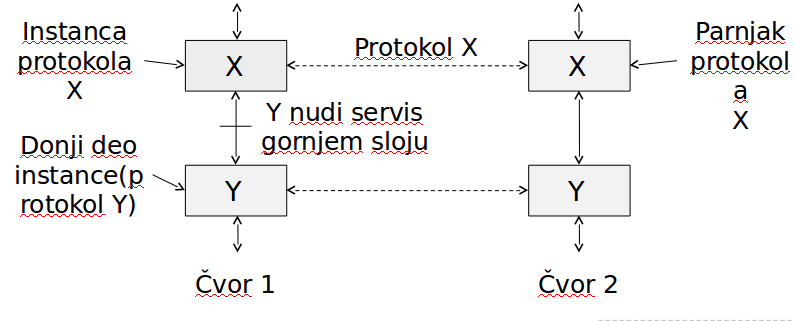
\includegraphics[width=9cm, height=5cm]{protokoli}\\
\end{center}

\subsection{Enkapsulacija}
Enkapsulacija je mehanizam slaganja slojeva protokola. Niži sloj pravi omotač oko sadržaja višeg sloja i dodaje svoje sopstvene informacije poruci. Sadržaj nižih slojeva je bliži spoljašnosti poruke. \\
\begin{center}
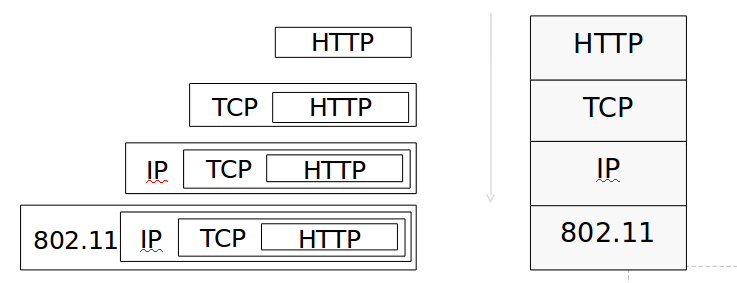
\includegraphics[width=9cm, height=4cm]{enkapsulacija}\\
\end{center}
Zahtev koji HTTP protokol definiše šalje se nižem sloju. TCP protokol dodaje svoja zaglavlja i skup informacija (metainf.) postaje sve veći kako se spuštamo po slojevima (to su enkapsulirane informacije). Zaglavlje sadrži upravljačke podatke, npr. zaglavlje jednog sloja može da sadrži redne brojeve koji omugućavaju tom istom sloju na drugom računaru da poruke isporuči ispravnim redosledom, za slučaj da niži slojevi taj redosled ne poštuju. Mogu da sadrže i veličine, vremena i druga polja. Sa svim tim informacijama se na poslednjem sloju poruka šalje na drugu stranu. Sad se informacije otpakuju, tj. primenjuje se inverzna funkcija za svaki od slojeva (uklanja se zaglavlje za svaki od slojeva) i kad se stigne do HTTP-a, on rekonstruiše originalnu poruku. \\
Smer toka podataka: $ \downarrow $(spušta se niz slojeve), zatim $ \rightarrow $
(prenosi se na najnižem sloju), pa $ \uparrow $ (podiže se uz slojeve).
\\
Protokol stek mora da bude poznat drugoj strani da bi bilo poznato kako treba da se otpakuje i svaki protokol zna samo svoju inverznu funkciju. Na drugoj strani, kada se poruka otpakuje, eliminišu se zaglavlja na svakom od slojeva i to se zove davanje usluge višim slojevima.\\
 Kada je nepogodno ili skupo da se za svaki par proces koji međusobno komuniciraju uspostavlja zasebna veza, odgovarajući sloj može da istu vezu upotrebi za više istovremenih, nezavisnih konverzacija. Sve dok je ovo \textit{multipleksiranje i demultipleksiranje} nevidljivo, može ga koristiti svaki sloj. Multipleksiranje je neophodno u fizičkom sloju gde se saobraćaj za sve veze mora preneti preko najviše nekoliko fizičkih linija. (kod njega na slajdovima stoji nešto za demultipleksiranje!)
 \\
\subsection{Prednosti raslojavanja}
- Prikrivanje informacija i ponovna upotreba\\
- Povezivanje različitih sistema\\
Šta se dešava ako imamo različite protokole na jednoj i na drugoj strani? Primer je slanje poruke sa uređaja zakačenog na WiFi na uređaj zakačenn na Ethernet. Tada na najnižim slojevima postoje tablice preslikavanja protokola. Poruka se samo prepakuje na poslednjem nivou. \\
\subsection{Mane raslojavanja}
- Povećani troškovi memorije i obrade (overhead)\\
Košta nas da dodajemo metapodatke. Manje bitno za duže poruke jer ne moramo svaki paket da dekorišemo. Početni i poslednji paket imaju veći broj informacija od središnjih, ali svaki paket ima dovoljno informacija da stigne na drugu stranu. Ne mora da budu početni i poslednji paket paketi koji imaju više informacija, mogu to biti i neki specijalni paketi. \\
- Prikrivanje informacija\\
Generalno je korisno, ali neke aplikacije žele da znaju da li se informacije prenose bežično ili putem kabla.


\section{Referentni modeli protokola i slojeva, jedince podataka, organizacije za standarde}
Ključno pitanje dizajna modela jeste koje funkcionalnosti implementira svaki od slojeva i koliko slojeva treba da postoji. Referentni modeli odgovaraju na ovakva pitanja. 
\subsection{OSI model sa 7 slojeva}

Internacionalan standard za povezivanje sistema. Uticajan ne, ali ne previše korišćen u praksi.
\\\\
1. \textbf{Fizički sloj}\\
Ima ulogu slanja \textit{bitova} putem realnih fizičkih komunikacionih kanala. U probleme njegovog projektovanja spada obezbeđivanje da kada jedna strana pošalje bit 1, druga strana takođe primi bit 1, a ne bit 0.\\\\
2. \textbf{Sloj veze podataka}\\
Ima ulogu slanja \textit{okvira}, odnosno skupova podataka. Pošiljalac ulazne podatke deli na okvire podataka, najčešće od po nekoliko stotina do nekoliko hiljada bajtova i okvire šalje jedan za drugim. Ako je usluga pouzdana, primalac potvrđuje ispravan prijem svakog okvira šaljući pošiljaocu okvir za potvrdu.
Jedan od problema koji se javlja u ovom sloju jeste neusaglašenost brzine slanja i brzine primanja podataka.\\\\
3. \textbf{Mrežni sloj}\\
Ima ulogu adresiranja, rutiranja \textit{paketa} i kontrole saobraćaja. Pri njegovom projektovanju ključno je odrediti kako se paketi upućuju od izvora ka odredištu. Putanje se mogu zasnivati na statičnim tabelama koje su ugrađene u mrežu i retko se menjaju. Jedan od zadataka ovog sloja je da omogući povezivanje heterogenih mreža.\\\\
4. \textbf{Transportni sloj}\\
Ima ulogu dostavljanja \textit{segmenata} (segmentacija, potrvđivanje). Osnovni zadatak je da prihvata podatke odzgo i da ih po potrebi razvrstava u manje grupe i da ih prosleđuje mrežnom sloju, obezbeđujući da svi delovi ispravno stignu na odredište. On takođe definiše usluge koje se nude sloju sesije.\\\\
5. \textbf{Sloj sesije}\\
Ima ulogu upravljanja sesijama.Omogućava korisnicima na različitim računarima da međusobno uspostave sesiju. Sesije nude različite usluge, uključujući upravljanje dijalogom, tj. vođenje računa o tome na koga je red da šalje poruke, rad sa žetonima, tj. sprečavanje učesnika da istovremeno pokrenu istu kritičnu operaciju i sinhronizovanje, tj. proveravanje dugačkog niza podataka tokom prenosa da bi se omogućilo nastavljanje od tačke prekida u slučaju pada sistema.\\\\
6. \textbf{Sloj prezentacije}\\
Ima ulogu konverzija za različite prezentacije. Bavi se sintaksom i semantikom prenetih informacija. Da bi računari koji podatke predstavljaju na različit način mogli da komuniciraju, strukture podataka koji se prenose mogu se definisati na apstraktan način i standardno kodirati u cilju prenosa. Sloj prezentacije obrađuje te apstraktne strukture podataka.\\\\
7. \textbf{Sloj aplikacije}\\
Ima funkcije potrebne korisniku, rad sa \textit{porukama}.  
\\
\\
Mana ovog modela jeste to što su  slojevi sesije i prezentacije gotovo prazni dok su sloj veze podataka i mrežni sloj prenatrpani.


\subsection{Internet referentni model}
Model sa 4 sloja, zasnovan na praksi. Sva tri gornja sloja se stapaju u jedan.
1. \textbf{Veza}\\
Ima ulogu fizičkog slanja podataka putem medijuma.Sam protokol za povezivanje s mrežom nije definisan i menja se od računara do računara i od jedne mreže do druge. \\\\
2. \textbf{Internet}\\
Ima ulogu slanja paketa putem raznorodnih mreža. Definiše Inernet protokol. Zadatak je da isporuči IP pakete tamo gde treba da stignu. Ovde je najveći problem problem usmeravanja i izbegavanja zagušenja.\\\\
3. \textbf{Transport}\\
Ima ulogu razmene podataka između čvorova. On je namenjen konverzaciji između ravnopravnih procesa na izvornom i odredišnom računaru, kao i transportni OSI sloj. Ovde su definisana dva protokola, protokol za upravljanje prenosom - TCP i protokol za korisničke datagrame - UDP. \\
TCP je pouzdan protokol sa uspostavljanjem direktne veze. Deli početni tok bajtova na zasebne poruke i svaku prosleđuje međumrežnom sloju. Prihvatni TCP proces na odredištu uređuje primljene poruke i od njih ponovo obrazuje tok bajtova. On upravlja i tokom podataka tako da brzi pošiljalac ne može da zatrpa sporog primaoca s više poruka nego što ovaj može da obradi. \\
UDP  predstavlja nepouzdan protokol bez uspostavljanja direktne veze namenjen aplikacijama koje same uređuju svoje pakete i upravljaju tokom podataka.\\\\
4. \textbf{Aplikacija}\\
Programi koji koriste usluge mreže. Sadrži sve protokole višeg nivoa - FTP za prenos datoteka, SMTP za elektronsku poštu, TELNET za virtuelni terminal koji omugućava korisniku da se sa svog računara daljinski prijavi na drugi računar i da na njemu radi, DNS za imenovanje domena, tj. za preslikavanje imena računara u njihove mrežne adrese, HTTP protokol za preuzimanje strana sa Worl Wide Weba i mnogi drugi.
\\\\
IP sloj je najtanji po pitanju broja protokola.

\begin{center}
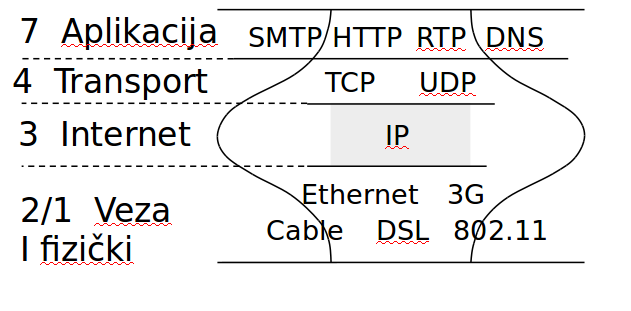
\includegraphics[width=9cm, height=4cm]{InternetRefModel}\\
\end{center}

Mana ovog modela jeste da on nije dovoljno uopšten, na primer, opisati Bluetooth pomoću ovog modela je sasvim nemoguće. Još jedna mana je to što ne razdvaja fizički sloj i sloj veze podataka. Ta dva sloja su potpuno različita. \\
\\

Mi ćemo koristiti hibridni model sa 5 slojeva: fizički sloj (bit), sloj veze (okvir), mrežni sloj (paket), transportni (segment) i aplikativni sloj (poruka). Jedinice podataka za svaki od slojeve su navedene u zagradama.\\
\\
Nazivi nekih uređaja u mreži: \\
- hab ili razvodnik ponavlja fizički signal na sve izlaze\\
- svič ili skretnica usmerava pakete samo onima kojima su potrebni, znači čita adresu\\
- ruter ili usmerivač usmerava pakete ali vodi računa i o dobrim putanjama\\\\

Neke poznatije organizacije za standarde:\\

\begin{center}
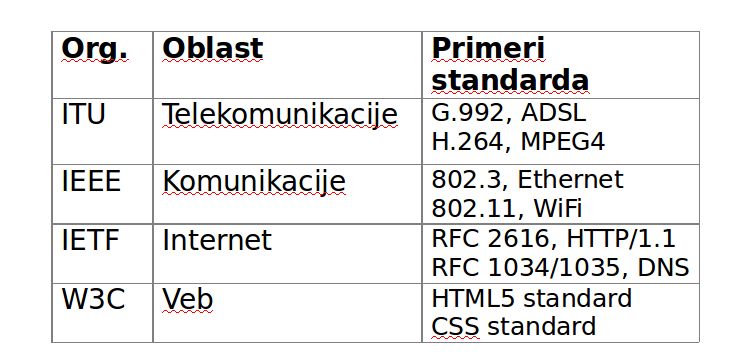
\includegraphics[width=9cm, height=4cm]{organizacije}\\
\end{center}
(Ovde kaže da treba i poglavlja 1.6 i 1.7, ali ja ne znam da li tu ima bilo šta bitno.)

\section{Fizički sloj, uloga, pojednostavljeni model, kašnjenja, BDP, primeri}
Tiče se slanja poruka putem komunikacionog kanala. Žice šalju analogni, tj. fizički signal, a mi želimo da šaljemo bitove koji su digitalni. Osnovna svrha je da niz bitova prenese bez greške s jednog računara na drugi. Za prenos mogu da se koriste različiti fizički medijumi. 
\subsection{Pojednostavljeni model}
Karakteristike uopštenog fizičkog kanala koje utiču na to koliko je kanal dobar:\\
- \textbf{\textit{protok}} (ili brzina, kapacitet) meren kao bitovi po sekundi b/s, označimo ga sa B\\
- \textbf{\textit{kašnjenje}} mereno u sekundama\\
Podrazumeva vreme potrebno da poruka stigne na ciljnu adresu. Označimo ga sa D. Postoje dve vrste kašnjenja, a to su: \\
1. \textit{Kašnjenje prenosa}, tj. vreme potrebno da se M-bitovna poruka postavi na komunikacioni kanal i različito je za sve kanale:
                 \begin{center}
                 T-delay = M (b) / B (b/s) = M/B s (sekundi)
                 \end{center}
2. \textit{Kašnjenje propagacije}, tj. vreme potrebno da bitovi prođu kroz komunikacioni kanal i slično je za sve kanale:
                  \begin{center}
           P-delay = dužina kanala/brzina signala (2/3 c) = X s (sekundi)
          *c – brzina svetlosti (nije svuda 2/3, različito za WiFi, optiku, ...)
                  \end{center}
Sabiranjem se dobija ukupno vreme.
                         \begin{center}
                         L = T+P = M/B + P
                         \end{center}
- \textbf{\textit{da li kanal emituje ili ne}}\\
- \textbf{\textit{raspodela verovatnoća grešaka}}\\
Primeri izračunavanja kašnjenja: \\
“Dialup” sa telefonskim modemom (slanje ka računaru u istom gradu npr):
                    \begin{center}
               P = 5 ms, B = 56 kb/s, M = 1250 B\\
              
               L = 5 ms + (1250x8)/(56 x 103) s = 5 ms+179 ms = 184 ms
                      \end{center}
Dugačka veza ili mali protok proizvode veće kašnjenje. Obično je jedna od komponenti kašnjenja P ili T dominantna.
\subsection{Protok-kašnjenje proizvod BDP}
BDP jeste proizvod protoka i vremena kašnjenja.
                     \begin{center}
                       BDP = B x D
                      \end{center}
Poruke zauzimaju prostor na kanalu. Količina podataka prisutnih na kanalu u nekom momentu je BDP. Ako bismo posmatrali podatak kao materiju, onda je ovo zapremina, tj. količina materije BDP = B x D. Meri se u bitovima i BDP je mali za kanale u lokalnim mrežama, npr. WiFi, a veliki za velike debele kanale.\\
\textbf{BDP primer}:\\
Slanje npr. od Perta do Sidneja preko optičkog kanala koji je dugačak.\\
B=40 Mb/s, D=50 ms $ \Rightarrow $ BDP = 40 x $10^{6}$ x 50 x $10^{-3}$ b = 2000 Kb = 250 KB\\
Ovo se smatra velikim BDP-om.\\
\\
Medijum propagira signal sa informacijama u vidu bitova. Tri osnovna tipa medija su: \\
- žičani\\
- optički (optički kablovi)\\
- bežični

\section{Žičani i optički komunikacioni medijumi}
Prednost je što se lako projektuje fiksni protok duž odabranih ruta, a mane su da je skup za postavljanje, posebno na većim udaljenostima i nije projektovan za mobilnost ili emitovanje.
\subsection{Žičani}
\subsubsection{Upredena parica}
Veoma česta, koristi se za LAN kablove i kod telefonskih linija.  Čine je dve izolovane bakarne žice, najčešće prečnika oko 1mm. Žice su međusobno spiralno uvijene, kao molekul DNK. Uvrtanjem se umanjuju smetnje. Najčešće se koristi u telefonskom sistemu, skoro svi telefoni su sa telefonskom centralom povezani uporednom paricom. Kada se veliki broj paralelnih parica protežu na veću daljinu, na primer sve linije iz jednog stambenog bloka do telefonske  centrale, one se povezuju u snop i obavijaju zaštitnim omotačem. Njome se mogu prenositi i analogni i digitalni signali. Brzina prenosa zavisi od debljine žice i rastojanja, ali se za daljine od nekoliko km u većini slučajeva može postići brzina od više megabita u sekundi.\\
Uporedna parica se realizuje u više oblika, od kojih su dva važna za računarske mreže. \\
- uporedna parica 3. kategorije se sastoji od dve blago uvijene izolovane žice. Četiri takva para obično se grupišu u zajedničkom plastičnom omotaču koji ih drži zajedno i štiti. \\
- uporedna parica 5. kategorije koje liče na parice 3. kategorije, ali su gušće upredene, čime je omogućen kvalitetniji signal na većim razdaljinama zbog čega su pogodnije za brzu komunikaciju između računara. \\
Uporedna parica 5. kategorije:
\begin{center}
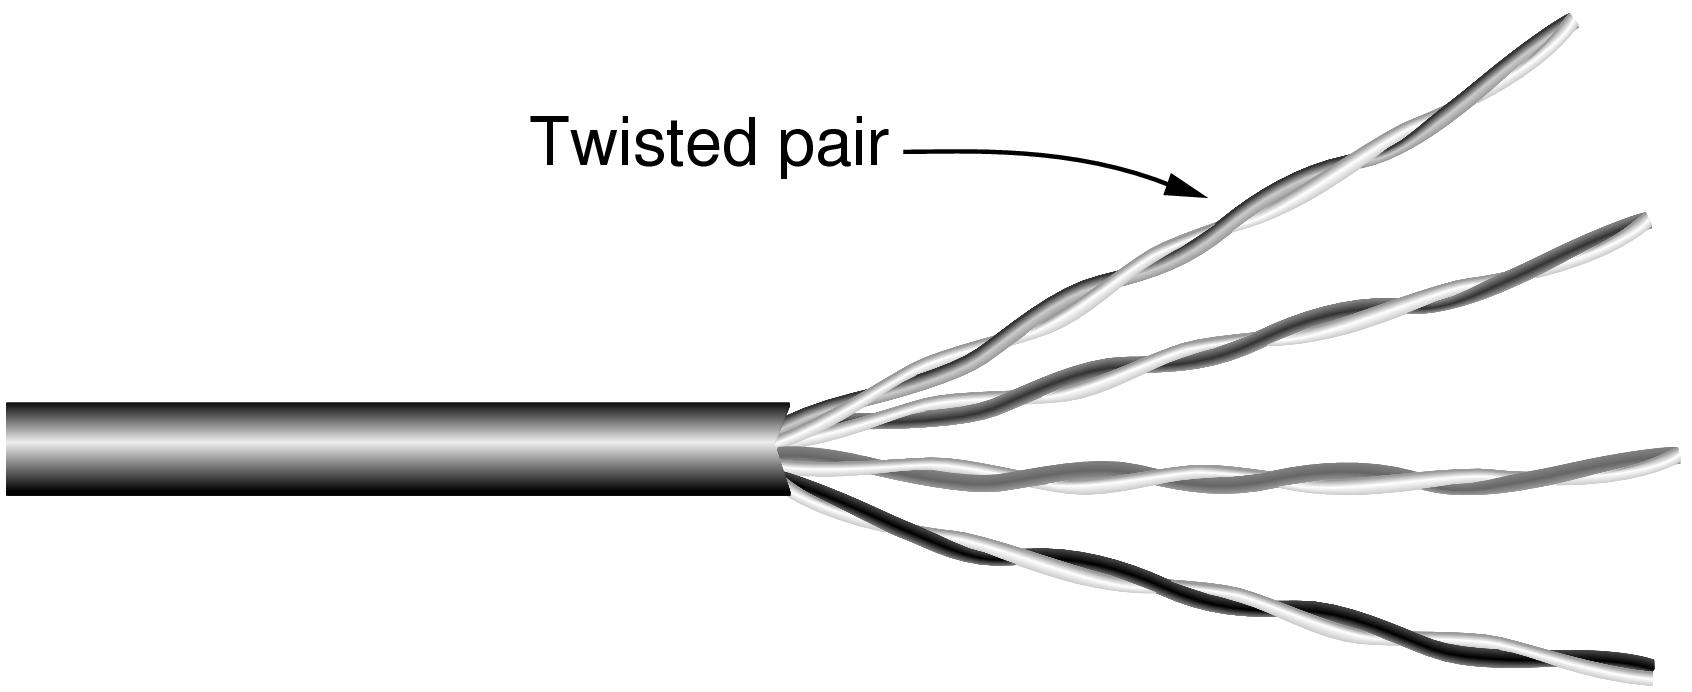
\includegraphics[width=7cm, height=3cm]{parica}\\
\end{center}

\subsubsection{Koaksijalni kabl}
Takođe čest. Daje bolju zaštitu i bolje performanse. Podatke prenosi većom brzinom i na veće daljine u odnosu na uporedne parice. Koriste se 50-omski i 75-omski koaksijalni kabl. Prvi se namenjuje digitalnom prenosu podataka, a drugi se koristi za prenos analognih podataka i za kablovsku televiziju, ali postaje sve važniji i za kablovski Internet. \\
Ovaj kabl ima jezgro od čvrste bakarne žice oko koje se nalazi izolator. Oko izolatora je cilindrični provodnik napravljen od gusto upletene bakarne mrežice. Preko njega dolazi zaštitni plastični omotač. Presek koaks. kabla:
\begin{center}
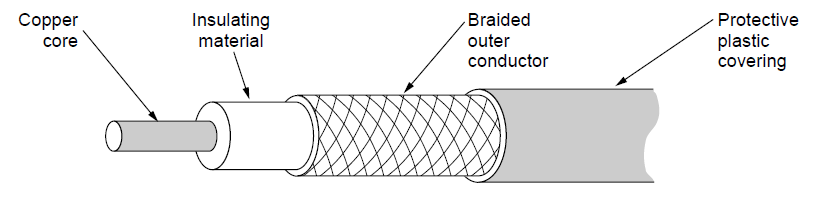
\includegraphics[width=12cm, height=3cm]{koaksijalni}\\
\end{center}
Savremeni koaks. kablovi imaju propusni opseg blizu 1GHz. Ranije su mnogo korišćeni za međugradske i međudržavne veze u telefonskim sistemima, ali su danas tu većinom zamenjeni optičkim kablovima. I dalje se koriste za kablovsku televiziju i gradske mreže.
\subsubsection{Instalacije za prenos struje}
Praktične za upotrebu jer već postoje. Jako loše karakteristike prenosa jer nisu dizajnirane za to.
\begin{center}
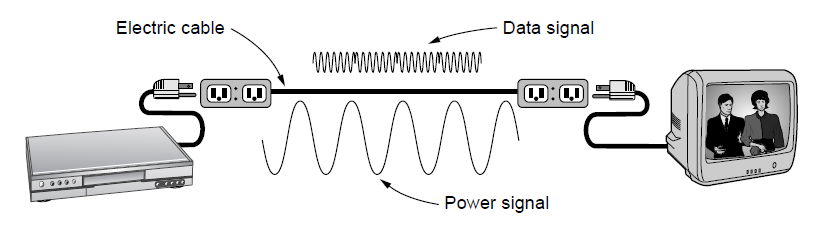
\includegraphics[width=12cm, height=3cm]{zicani}\\
\end{center}

\subsection{Optički}
Dugačka, tanka i čista vlakna stakla. Ogroman protok zbog opsega frekvencija. Velike udaljenosti zbog malog slabljenja. \\
Optički sistem za prenos podataka sadrži tri glavne komponente: svetlosni izvor, prenosni medijum i detektor. Po konvenciji, svetlosni impuls označava bit 1, a odsustvo impulsa označava bit 0. Prenosni medijum je ultratanko stakleno vlakno. Detektor proizvodi električni impuls kada na njega padne svetlosni zrak. Spajajući svetlosni izvor s jednim krajem optičkog vlakna, a detektor sa njegovim drugim krajem, dobijamo jednosmerni sistem prenosa podataka koji prihvata električni signal, pretvara ga u svetlosni impuls i prenosi, a zatim ga na drugom kraju pretvara u električni signal.
\begin{center}
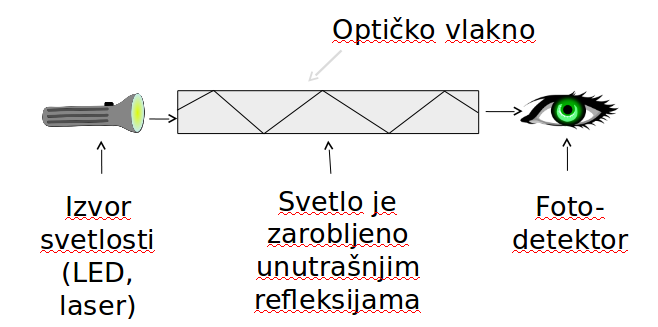
\includegraphics[width=9cm, height=4cm]{opticki1}\\
\end{center}
 Kada upadni ugao zraka pređe određenu kritičnu vrednost, zrak uopšte ne prelazi u vazduh, već se vraća u kvarc. Na taj način je zauvek zarobljen u vlaknu.\\
Slabljenje svetlosti pri prolasku kroz staklo zavisi od talasne dužine svetlosti, a i od izvesnih svojstava stakla. \\
Optički kablovi su slični koaks. kablovima samo što nemaju mrežasti provodnik.  Duž ose kabla proteže se stakleno jezgro kroz koje prolazi svetlosni zrak. Jezgro je okruženo oblogom od stakla čiji je indeks prelamanja manji od indeksa prelamaja jezgra kako bi se sva svetlost zadržala u jezgru. Oko svega se nalazi plastični omotač koji štiti oblogu. Vlakna se najčešće grupišu u snopove i zaštićuju dodatniim spoljim omotačem.
Koriste se za lokalne mreže i za prenos podataka na velika rastojanja. Polažu se na dubini od jednog metra ispod površine tla.\\

Pojedinačno vlakno i pakovanje vlakna:
\begin{center}
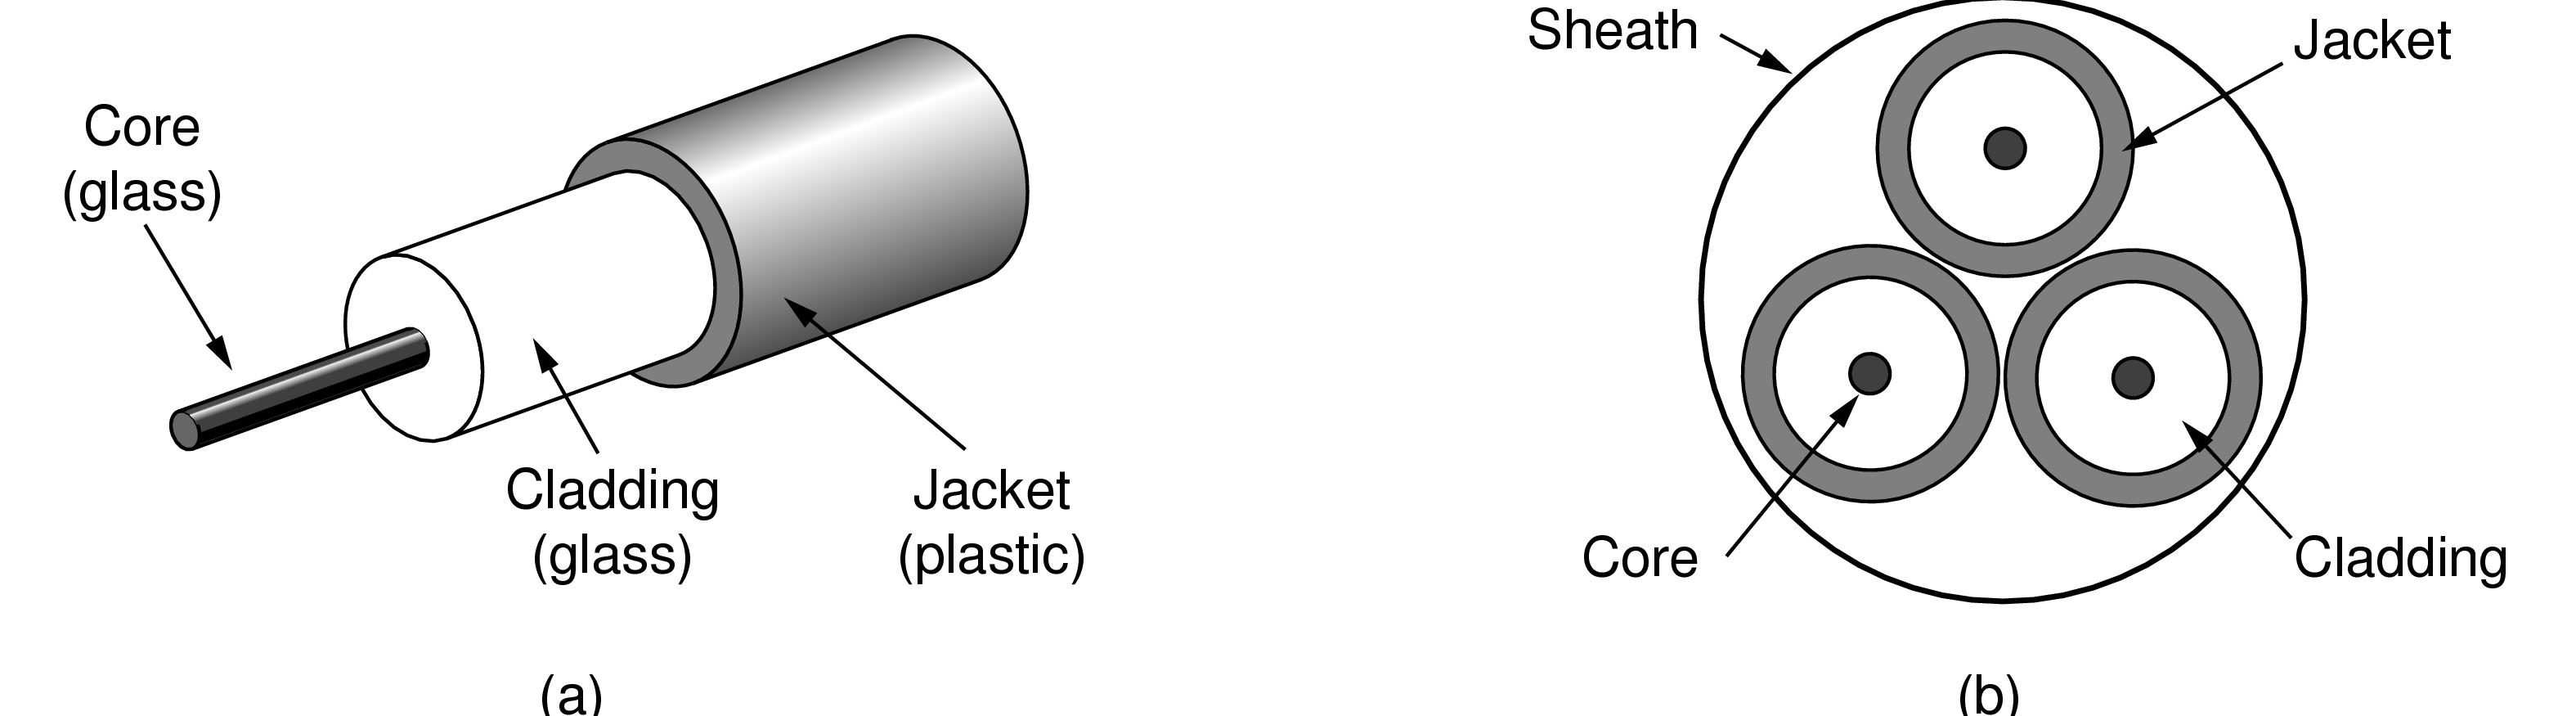
\includegraphics[width=12cm, height=3cm]{pojedinacno}
\end{center}

\subsubsection{Unimodalno vlakno}
Toliko je tanko da svetlost praktično ide pravo. Vlakno radi kao talasovod i svetlost se kroz njega prostire pravolinijski, bez odbijanja. Drugi naziv je jednorežimsko vlakno. Skuplja su od višerežimskih i koriste se za veća rastojanja. Mogu da prenose signale na daljinu od 100km, brzinom 50 Gb/s.
\begin{center}
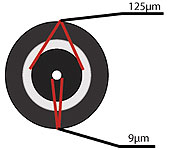
\includegraphics[width=3cm, height=2cm]{unimodalno}\\
\end{center}

\subsubsection{Višemodalno vlakno}
Kod ovog vlakna svetlost se sudara sa zidovima. Kroz vlakno može istovremeno prolaziti više svetlosnih zrakova od kojih se svaki odbija pod drugačijim uglom, uvek većim od kritične vrednosti. Za svaki zrak se kaže da kroz vlakno prolazi drugačijim režimom, pa se zbog toga zovu višemodalna ili višerežimska vlakna.
\begin{center}
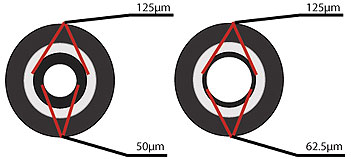
\includegraphics[width=5cm, height=2cm]{visemodalno}\\
\end{center}

\section{Bežični komunikacioni medijumi}
Prednosti su da prirodno podržavaju emitovanje, jednostavne za postavljanje i jeftine, prirodno podržavaju mobilnost, a mane su mešanje signala koje se mora razrešavati i to što jačina signala, pa samim tim i protok, izuzetno varira.\\
Pošiljalac emituje signal kroz prostor. Signal se emituje u svim pravcima za razliku od žice. Bliski signali, tj. signali slične frekvencije, se mešaju kod primaoca, pa je potrebno koordinirati upotrebu. Kako bi se izbegla mešanja signala, opsezi, tj. bandovi se pažljivo dodeljuju. Čak se prodaju na aukcijama za najviše ponude.\\
Za mreže je najinteresantniji opseg mikrotalasa (3G, 4G, WiFi), ali se koriste i ostali delovi spektra.\\
\begin{center}
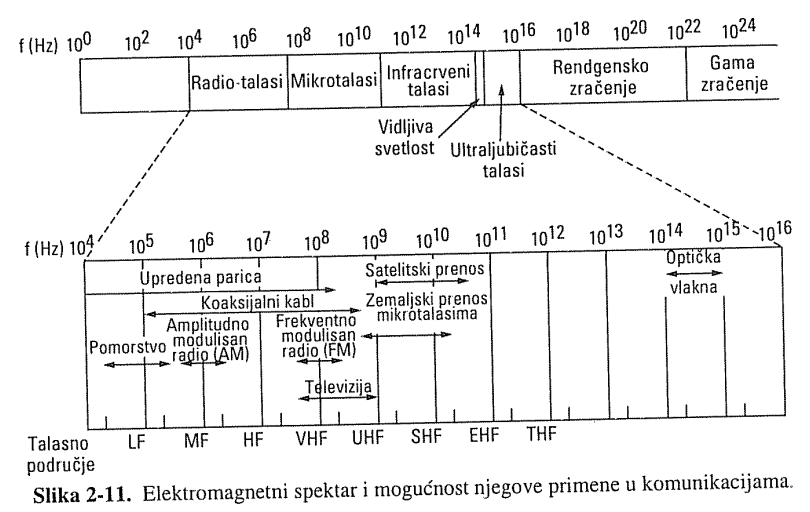
\includegraphics[width=10cm, height=6cm]{eltalasi}\\
\end{center} 
Drugačiji pristup od dodeljivanja frekvencija je da se one uopšte ne dodeljuju. Pusti se da svako po volji emituje, ali da se snaga emitovanja ograniči na mali radijus da emisije ne ometaju jedna drugu. U tom smislu, većina zemalja je odvojila određena talasna područja, zvana \textbf{industrijska, naučna i medicinska frekvencija} (\textit{Industrial, Scientific, Medical - ISM}) za nelicencirano korišćenje. Daljinski upravljači za garažna vrata, bežični telefoni, igračke i brojni drugi bežični kućni aparati koriste ISM područja.\\
Mikrotalasi, 3G i nelicencirane frekvencije (ISM) - obično zbog fragmentacije drugih bandova, npr. WiFi. (???? uzeto sa slajdova). Slika dole se odnosi na ovo.
\begin{center}
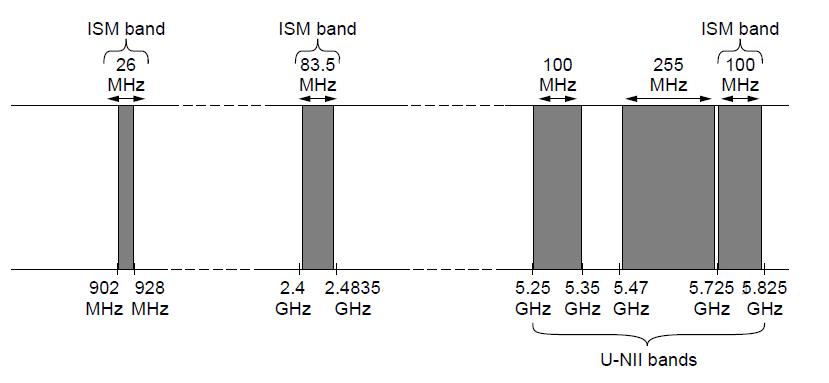
\includegraphics[width=10cm, height=4cm]{stagod}\\
\end{center} 

\subsection{Radio-talasi}
Radio-signali mogu da prolaze kroz zgrade, ali im signal slabi iz raznih razloga. Neki od razloga su to što biva apsorbovan ili zbog odbijanja. U opsezima VLF(very low freq.), LF(low freq.) i MF(medium freq.) radio-talasi prate zakrivljenost zemlje (ovi talasi lako prolaze kroz zgrade što omogućuje da se u njima slušaju tranzitorski prijemnici), a u HF(high freq.) opsegu se odbijaju od jonosfere i vraćaju se nazad, na Zemlju (što se koristi za komunikaciju radio-amatera na velikim rastojanjima). Radio-talasi se prostiru na sve strane od izvora, tako da položaj predajnika i prijemnika nije od velikog značaja.
\subsection{Mikrotalasi}
Imaju veliki frekventni opseg i koriste se često za zatvorene namene poput WiFi, kao i za otvorene poput 3G i sateliti. Mikrotalasi su talasi na frekvenciji iznad 100 MHz. Pošto se mikrotalasi prostiru pravolinijski (sva energija se koncentrise u uzak snop pomoću patabolične antene), zbog zakrivljenosti Zemlje, tornjevi ne smeju biti previše udaljeni. Što su tornjevi viši, rastojanje između njih može da bude veće. Mikrotalasi loše prolaze kroz zidove. Signal slabi i reflektuje se od objekata iz okruženja. Jačina varira zbog udaljenosti, sabiranja signala i slično. I kada se talasi dobro usmere na predajniku, oni se ipak na putu mogu rasuti. Neki talasi se mogu odbiti od niskih atmosferskih slojeva i zato na cilj stići kasnije od direktnih talasa. Zakasneli talas može da dođe u suprotnu fazu s direktnim talasom i da ga tako poništi. Taj efekat se zove \textit{slabljenje zbog različitih putanja}.
\subsection{Svetlost}
Svetlosni signali (ne misli se na optička vlakna) se mogu koristiti kao komunikacioni medijum. Svetlost je vrlo usmeren talas i ima veliki frekventni opseg (protok u elektroinženjerskom smislu).\\
Koristi se za povezivanje lokalnih mreža u dve zgrade pomoću laserskih uređaja na krovovima. Laserski zrak je po prirodi usmeren, tako da na svakoj od dve zgrade mora postojati i laser i fotodetektor. Takav sistem ima veoma veliku propusnu moć i izuzetno je jeftin. Za njega nije potrebno tražiti zvaničnu dozvolu vlasti, za razliku od mikrotalasa. \\
Nedostatak je što moć laserskog snopa ne može da prodre kroz kišu ili maglu, ali tokom sunačnih dana on radi odlično.
\begin{center}
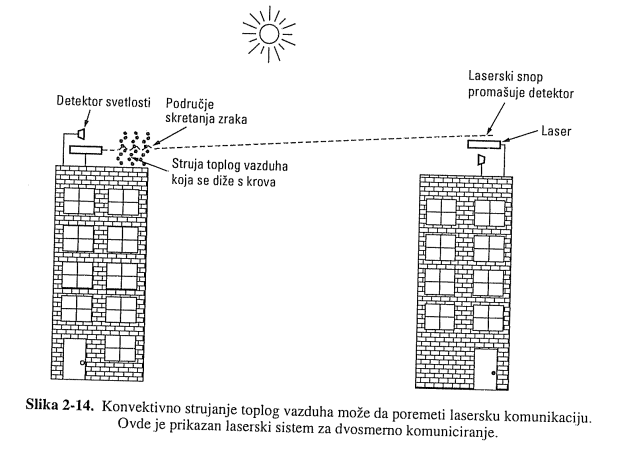
\includegraphics[width=12cm, height=8cm]{svetlost}\\
\end{center}

\section{Komunikacioni sateliti}
Sateliti su efikasni za emitovanje i komunikaciju bilo kada i bilo gde. \\
Kom. satelit može da se zamisli kao veliki repetitor na nebu koji sadrži više transpondera od kojih svaki osluškuje određeni deo elektromagnetnog spektra, pojačava primljeni signal i ponovo ga emituje na drugoj frekvenciji. \\
Tipovi satelita:
\begin{itemize}
  \item Geostacionarni (GEO)
  \item Srednje-orbitni (MEO)
  \item Nisko-orbitni (LEO)
\end{itemize}
\begin{center}
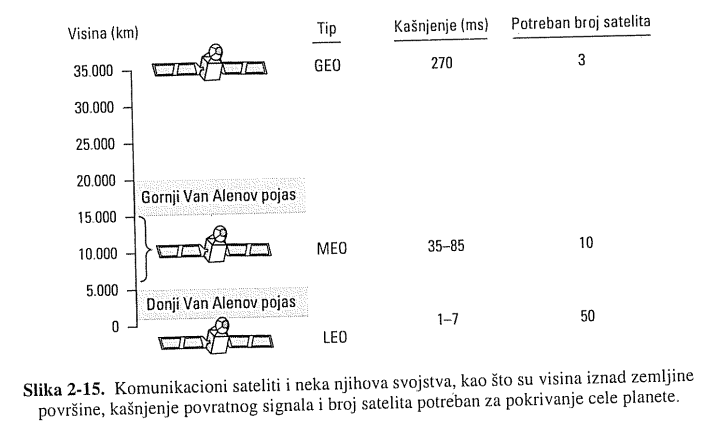
\includegraphics[width=12cm, height=8cm]{sateliti}\\
\end{center}
\subsection{Geostacionarni sateliti}
Orbitiraju 35000km iznad fiksne lokacije. Najnovije dostignuće na ovom polju jesu jeftine mikrostanice - \textbf{terminali s vrlo uskim emisionim snopom} (\textit{Very Small Aperture Terminals, VSATs}). U mnogim VSAT sistemima, mikrostanice nemaju dovoljnu snagu da direktno komuniciraju jedna s drugom (preko satelita), već se saobraćaj između njih odvija preko tzv. habova, ili razvodnika - zemaljske antene visokog učinka. VSAT dobija i šalje signal ka centralnom uređaju koji se naziva hab (postoje i sistemi bez centralizovanog uređaja). Hab, na primer, odašilja televizijski program ka GEO, a ovaj emituje na delu zahvaćene Zemljine teritorije, te ka svim pripadajućim VSAT uređajima. U ovakvom režimu rada, korišćenjem mikrostanica male snage, kašnjenje signala je veće.\\
\begin{center}
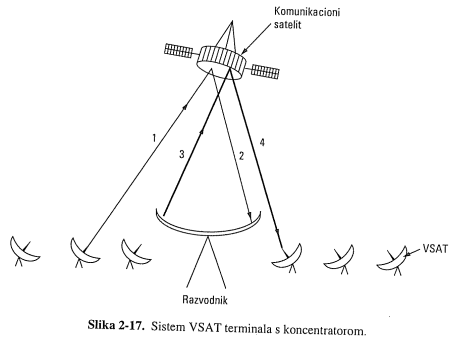
\includegraphics[width=12cm, height=8cm]{GEO}\\
\end{center}
Svojstvo satelitskog prenosa je i to što cena prenete poruke ne zavisi od udaljenosti. Prekookeanska veza košta kao i veza sa komšijom preko puta. Sa aspekta bezbednosti i privatnosi, sateliti su jako loši jer svako može sve da čuje. Neophodno je šifrovati podatke.
\subsection{Nisko-orbitni sateliti}
Nisu geostacionarni pa zbog toga što se brzo kreću mora da ih ima više kako bi mogli da garantuju stalnu pokrivenost na odabranim regijama. Brži odziv u odnosu na GEO jer su bliži Zemlji (kašnjenje signala iznosi nekoliko milisekundi). \\
\begin{center}
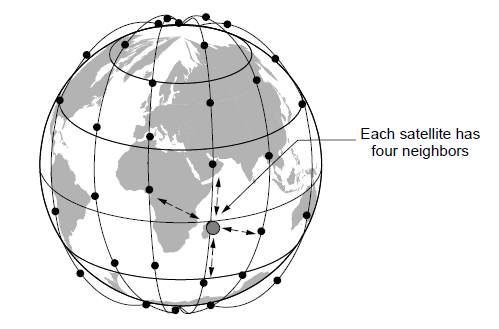
\includegraphics[width=8cm, height=5cm]{LEO}\\
\end{center}
Jedna vrsta ovakvih sistema je namenjena Internetu, a to je \textbf{Teledesic}. Cilj sistema bio je da se za milione korisnika Interneta obezbedi istovremena veza ka satelitu brzine do 100Mb/s, a od satelita do 720Mb/s. 
\subsection{Sateliti ili optika?}
Prednosti satelita su:
\begin{itemize}
  \item nakon lansiranja satelita, komunikacija može brzo da se uspostavi bilo gde i bilo kada
  \item emitovanje na velika područja
\end{itemize} 
Mane satelita su:
\begin{itemize}
  \item ograničen protok
  \item mešanje signala
\end{itemize}
Prenosti optike:
\begin{itemize}
  \item ogroman protok duž velikih udaljenosti
\end{itemize}
Mana optike:
\begin{itemize}
  \item instalacija skupa
  \item instalacija komplikovana
\end{itemize}

\section{Signali, prenos, frekvenciona reprezentacija, signal u žičanim, optičkim, bežičnim medijumima}
(pogledati knjigu 2.1.1 i 2.1.2 poglavlja)\\

Analogni signali kodiraju digitalne. Šta se dešava sa signalom prilikom propagacije?\\
Podaci se mogu prenositi žicom tako što se menja neko njeno fizičko svojstvo, npr. napon ili jačina struje. Kada predstavimo vrednost tog napona ili te jačine struje kao jednoznačnu funkciju vremena, f(t), možemo da modeliramo ponašanje signala i da ga analiziramo služeći se matematičkim metodama. \\

Signal se kroz vreme može predstaviti putem svojih frekvencijskih delova (Furijeova analiza).\\
Svaka normalna periodična funkcija $ g(t) $ periode $ T $ se može predstaviti kao zbir (možda beskonačnog) broja sinusnih i kosinusnih funkcija:
\begin{center}
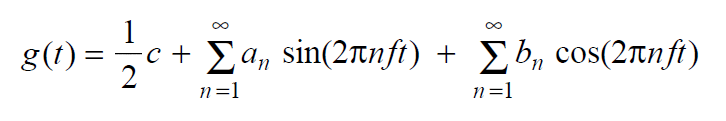
\includegraphics[width=10cm, height=2cm]{furije}\\
\end{center}
gde je $ f = 1/T $ osnovna frekvencija, $ a_{n} $ i $ b_{n} $ su amplitude $ n$-tog člana (harmonika) sinusne i kosinusne funkcije, a $c$ je konstanta. Tako razložena periodična funkcija naziva se \textbf{Furijeov niz}. Iz njega se može rekonstruisati prvobitna funkcija; to znači, ako je poznata perioda $T$ i ako su zadate amplitude prvobitna funkcija se dobija sabiranjem niza iz gornje jednačine.\\

Signal podataka koji ima ograničeno trajanje može se rastaviti u Furijeov niz ako zamislimo da se njegov profil stalno ponavlja, tj. da se profil iz intervala $0$ do $T$ istovetno ponavlja u intervalu od $T$ do $2T$, itd.\\

Amplitude $a_{n}$ mogu se izračunati za svaku funkciju $g(t)$ množenjem obe strane gornje jednačine činiocem $sin(2 \pi kft)$, a zatim integrisanjem jednačine u intervalu od $0$ do $T$. Slično tome, množeći gornju jednačinu sa $cos(2 \pi kft)$ i integrišući je između $0$ i $T$, možemo da dobijemo amplitudu $ b_{n} $. Neposrednom integracijom obe strane gornje jednačine  dobijamo $c$.
\begin{center}
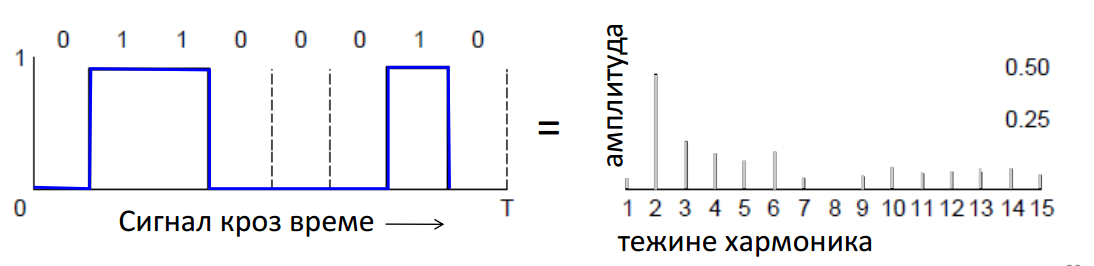
\includegraphics[width=12cm, height=3cm]{furije2}\\
\end{center}

Da bismo razumeli kakve veze ovo ima s prenosom podataka, razmotrimo jedan primer: slanje slova $b$ kodiranog pomoću 8 bitova. Niz bitova koje treba preneti izgleda ovako: 01100010. Leva strana gornje slike prikazuje napon signala koji šalje računar. Srednjekvadratne amplitude, za prvih nekoliko članova niza, prikazane su na desnoj strani slike. One su važne jer su njihovi kvadrati proporcionalni energiji koja se pri određenoj frekvenciji prenese. \\

Nema transportnog medijuma koji prenosi signale bez gubitaka. Kada bi sve komponente Furijeovog niza podjednako slabile, amplituda signala bila bi takođe manja, ali se signal ne bi izobličio, tj. imao bi isti pravougaoni oblik kao na gornjoj slici. Nažalost, u svim prenosnim medijumima različite komponente F. niza različito slabe, što dovodi do izobličenja signala. Opseg frekvencija koje se prenose bez većeg slabljenja naziva se \textbf{propusni opseg}. Često se definiše kao opseg frekvencija od 0 do frekvencije pri kojoj snaga signala opadne na polovinu.
\\

Manji skup frekvencija, manji protok:
\begin{center}
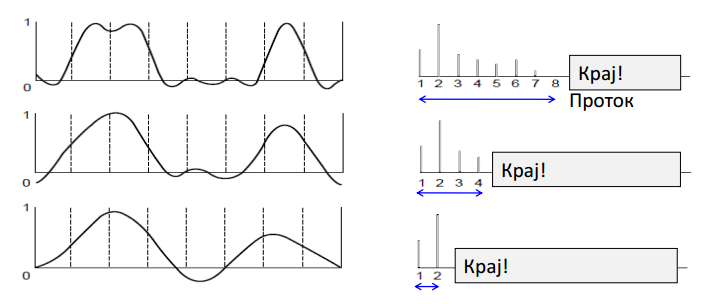
\includegraphics[width=12cm, height=6cm]{furije3}\\
\end{center}

Ograničavanjem propusnog opsega ograničava se i brzina prenosa, čak i kroz savršene kanale.\\
Elektroinženjeri: Protok  je širina frekv. opsega (Hz)\\
Računarci: Protok je kapacitet prenosa informacija (b/s)

\subsection{Signal preko žice}
Šta se dešava sa signalom dok prelazi kroz žicu?
\begin{itemize}
  \item signal kasni (brzina je ~$2/3c$, a ne beskonačna)
  \item signal slabi (sa porastom udaljenosti)
  \item frekvencije iznad neke granice brže slabe
  \item dešava se šum (zbog spoljnih efekata)
\end{itemize}
\begin{center}
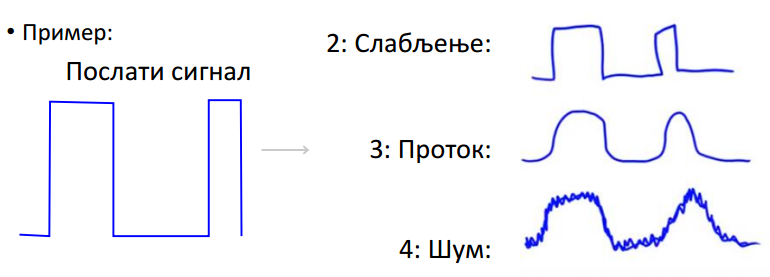
\includegraphics[width=15cm, height=5cm]{protok1}\\
\end{center}

\subsection{Signal preko optike}
Svetlo se prenosi sa veoma malim gubitkom u tri široka frekventna opsega. Krajni desni zalazi u opseg infracrvenih talasa.
\begin{center}
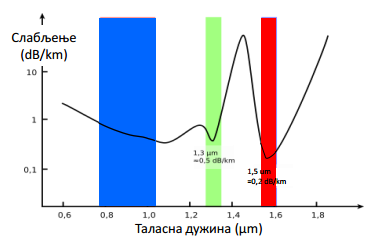
\includegraphics[width=8cm, height=5cm]{protok2}\\
\end{center}

\subsection{Signal u bežičnim komunikacijama}
Zbog visokih frekvencija bežičnih prenosa, nije moguće digitalni signal direktno kodirati u analogni, već se koristi koncept \textbf{signala nosača}.
\begin{center}
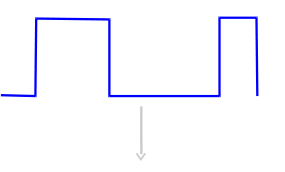
\includegraphics[width=3cm, height=2cm]{signal}\\
\end{center}
\begin{center}
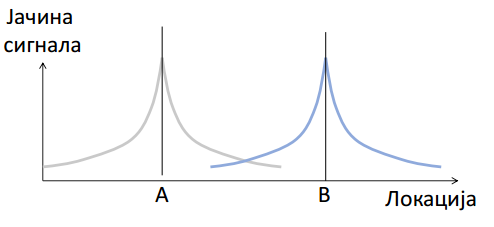
\includegraphics[width=6cm, height=3cm]{signal2}\\
\end{center}
Putuje brzinom svetlosti, ali jako brzo slabi (sa kvadratom rastojanja, zašto?)\\

Višestruki signali na istoj frekvenciji se mešaju kod primaoca. Ako su lokacije dovoljno udaljene, moguće je koristiti istu frekvenciju.
\begin{center}
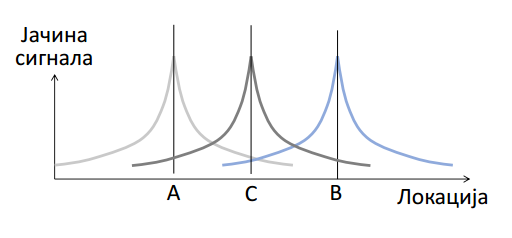
\includegraphics[width=6cm, height=3cm]{signal3}\\
\end{center}
Postoje još neki otežavajući efekti. Propagacija bežičnog signala je složena i zavisi od okruženja. Karakteristike zavise i od frekvencije. Ne prenosi se isto zvuk i svetlost, u čemu je razlika? Postoji problem sa \textit{sabiranjem odbijenih signala} kod mikrotalasa. Signali mogu da se odbijaju od objekta i putuju kroz više nezavisnih putanja. Posle, kada stignu višestruki signali kod primaoca, oni se mogu loše sabrati.  Primer:
\begin{center}
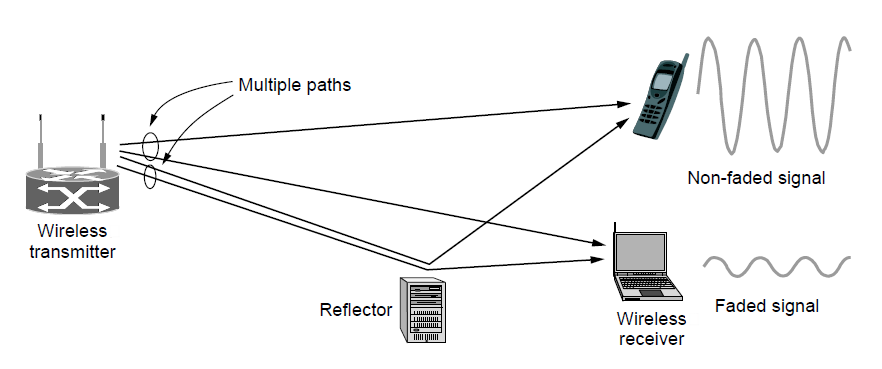
\includegraphics[width=10cm, height=4cm]{signal4}\\
\end{center}

\section{Modulacija i multipleksiranje signala}
Sa slajdova i u knjizi poglavlje.


\section{Prirodna ograničenja prenosa signala}
Čak i savršen kanal ima ograničen kapacitet prenosa.
Koliko često se može slati podatak kroz kanal? O tome govore Najkvistov limit i Šenonov kapacitet. Realni sistemi su dobro realizovani ako nisu mnogo daleko od ovih ograničenja. Ograničenja nam govore koliko smo relativno dobri u nečemu.\\
Protok - B, jačina, tj. snaga signala - S, jačina, tj. snaga šuma - N. B ograničava brzinu promena - frekvenciju i to je karakteristika kanala. S i N ograničavaju broj razlučivih nivoa signala i to je karakteristika primaoca.\subsection{Najkvistov limit}
Maksimalan broj promena simbola je 2B (101010101010101010..). Ako postoji V nivoa signala (ignorišemo greške, tj. šum), onda je maksimalan protok u bitima, tj. najveća brzina prenosa:
\begin{center}
 $ R=2B log_{2} V$  b/s.
\end{center}
Ovo je jednačina za maksimalnu brzinu prenosa kroz bešumni kanal ograničene propusne moći. \\
Na primer, bešumni kanal propusnog opsega 3 kHz ne može da prenosi binarne signale brzinom većom od 6000 b/s.

\subsection{Šenonov kapacitet}

Proširenje Najkvistove jednačine na kanale sa slučajnim, tj. termičkim šumom. Termički šum uvek postoji zbog kretanja molekula u sistemu. Izražava se kao količnik snage signala i snage šuma i naziva se  odnos \textbf{signala i šuma - SNR }, odnosno S/N. Broj razlučivih nivoa signala zavisi od S/N. SNR se meri u decibelima: $ SNR_{dB} = 10 log_{10} S/N $. Ako je SNR jednak 10, onda je $SNR_{dB} $ jednak 10, ako je SNR jednak 100, onda je $ SNR_{dB} $ jednak 20, itd. Koristi se logaritamska skala jer S/N može jako mnogo da varira.\\
Šenonova jednačina:
\begin{center}
 $ C=B log_{2} (1+S/N)$  b/s.
\end{center}
Broj razlučivih signala se dobija iz odnosa $ (S+N)/N = 1+S/N $.
\\
Na primer, kanal propusnog opsega 3000Hz, sa odnosom signala i termičkog šuma 30dB neće nikada moći da prenosi podatke brzinom većom od 30000b/s, bez obzira na broj naponskih nivoa signala ili učestalost uzorkovanja. Šenon je postavio gornju teorijsku granicu - realni sistemi je retko dostižu.
\\\\\\\\
Žice i optika: mogu se projektovati ciljni SNR i B, a samim tim i ciljni prenos u b/s.\\
Bežični kanali: Za dato B, SNR drastično varira, čak i do 60dB. Nije isplativo projektovati za najgori slučaj, mora se živeri sa visokim varijacijama prenosa.

\section{Pregled relevantnijih sistema komunikacija}
\section{Sloj veze, uloga, komunikacija sa slojem ispod i iznad, kratko objašnjenje spiska aktivnosti na sloju veze}
\section{Uokvirivanje u sloju veze}
\section{Kodiranje grešaka u sloju veze}
\section{Detekcija grešaka u sloju veze}
\section{Korekcija grešaka u sloju veze}
\section{Sloj veze, tipovi servisa, okruženje, utopijski jednosmerni protokol}
\section{Kontrola toka, ARQ, pauze (tajmauti), duplikati, protokol „stani i čekaj“ za savršen i nesavršen kanal}
\section{Protokol kliznih prozora u sloju veze, „1-bitni“, „vrati se N“, „selektivno ponavljanje“}
\section{MAC podsloj, uloga, alokacija kanala, ALOHA protokol}
\section{CSMA, CSMA/CD, BEB}
\section{MAC protokoli zasnovani na redosledu, Token Ring}
\section{MAC protokoli za bežične mreže}
\section{Klasični Eternet}
\section{Moderni (komutirani) Eternet. i na sloju veze}

\end{document} % The document ends here